%%
%% This is file `sample-authordraft.tex',
%% generated with the docstrip utility.
%%
%% The original source files were:
%%
%% samples.dtx  (with options: `authordraft')
%% 
%% IMPORTANT NOTICE:
%% 
%% For the copyright see the source file.
%% 
%% Any modified versions of this file must be renamed
%% with new filenames distinct from sample-authordraft.tex.
%% 
%% For distribution of the original source see the terms
%% for copying and modification in the file samples.dtx.
%% 
%% This generated file may be distributed as long as the
%% original source files, as listed above, are part of the
%% same distribution. (The sources need not necessarily be
%% in the same archive or directory.)
%%
%% The first command in your LaTeX source must be the \documentclass command.
\documentclass[sigconf,authordraft]{acmart}


%%%% As of March 2017, [siggraph] is no longer used. Please use sigconf (above) for SIGGRAPH conferences.

%%%% As of May 2020, [sigchi] and [sigchi-a] are no longer used. Please use sigconf (above) for SIGCHI conferences.

%%%% Proceedings format for SIGPLAN conferences 
% \documentclass[sigplan, anonymous, authordraft]{acmart}

%%%% Proceedings format for conferences using one-column small layout
% \documentclass[acmsmall,authordraft]{acmart}

%% 追加
\usepackage{bm}
\newcommand\figref[1]{\textbf{Figure~\ref{fig:#1}}}
\newcommand\tabref[1]{\textbf{Table~\ref{tab:#1}}}
\usepackage{url}
\usepackage{color}
%% ここまで

% NOTE that a single column version is required for submission and peer review. This can be done by changing the \doucmentclass[...]{acmart} in this template to 
% \documentclass[manuscript,screen]{acmart}

%%
%% \BibTeX command to typeset BibTeX logo in the docs
\AtBeginDocument{%
  \providecommand\BibTeX{{%
    \normalfont B\kern-0.5em{\scshape i\kern-0.25em b}\kern-0.8em\TeX}}}

%% Rights management information.  This information is sent to you
%% when you complete the rights form.  These commands have SAMPLE
%% values in them; it is your responsibility as an author to replace
%% the commands and values with those provided to you when you
%% complete the rights form.
\setcopyright{acmcopyright}
\copyrightyear{2018}
\acmYear{2018}
\acmDOI{10.1145/1122445.1122456}

%% These commands are for a PROCEEDINGS abstract or paper.
\acmConference[Woodstock '18]{Woodstock '18: ACM Symposium on Neural
  Gaze Detection}{June 03--05, 2018}{Woodstock, NY}
\acmBooktitle{Woodstock '18: ACM Symposium on Neural Gaze Detection,
  June 03--05, 2018, Woodstock, NY}
\acmPrice{15.00}
\acmISBN{978-1-4503-XXXX-X/18/06}


%%
%% Submission ID.
%% Use this when submitting an article to a sponsored event. You'll
%% receive a unique submission ID from the organizers
%% of the event, and this ID should be used as the parameter to this command.
%%\acmSubmissionID{123-A56-BU3}

%%
%% The majority of ACM publications use numbered citations and
%% references.  The command \citestyle{authoryear} switches to the
%% "author year" style.
%%
%% If you are preparing content for an event
%% sponsored by ACM SIGGRAPH, you must use the "author year" style of
%% citations and references.
%% Uncommenting
%% the next command will enable that style.
%%\citestyle{acmauthoryear}

%%
%% end of the preamble, start of the body of the document source.
\begin{document}

%%
%% The "title" command has an optional parameter,
%% allowing the author to define a "short title" to be used in page headers.
\title{User Identification Method based on Head Shape using a Helmet with Pressure Sensors}

%%
%% The "author" command and its associated commands are used to define
%% the authors and their affiliations.
%% Of note is the shared affiliation of the first two authors, and the
%% "authornote" and "authornotemark" commands
%% used to denote shared contribution to the research.
\author{Atsuhiro Fujii}
\affiliation{%
  \institution{Ritsumeikan University}
  \city{Shiga}
  \country{Japan}}
\email{atsuhiro.fujii@iis.ise.ritsumei.ac.jp}

\author{Kazuya Murao}
\affiliation{%
  \institution{Ritsumeikan University}
  \city{Shiga}
  \country{Japan}}
\email{murao@cs.ritsumei.ac.jp}

%%
%% By default, the full list of authors will be used in the page
%% headers. Often, this list is too long, and will overlap
%% other information printed in the page headers. This command allows
%% the author to define a more concise list
%% of authors' names for this purpose.
\renewcommand{\shortauthors}{Fujii and Murao}

%%
%% The abstract is a short summary of the work to be presented in the
%% article.
\begin{abstract}
Various types of helmets exist, including industrial protective helmets, motorcycle helmets, sports helmets, and military/police helmets. By identifying individuals wearing a helmet, their name, affiliation, and qualification can be presented on a display mounted on the helmet, and sensor data collected through the helmet, such as acceleration, video, and eye-tracking data, can be labeled with the user's ID. In this paper, we propose a user identification method based on head shape using a helmet equipped with 32 pressure sensors.
%Our method has two functions: user identification and authentication. Identification aims to classify a user as a registered user, while authentication aims to accept users who are registered in the system and reject unknown users.
We implemented a prototype helmet device and collected data from nine subjects, resulting in 100\% accuracy for user identification and an average equal error rate of 0.076 for user authentication.
\end{abstract}

%%
%% The code below is generated by the tool at http://dl.acm.org/ccs.cfm.
%% Please copy and paste the code instead of the example below.
%%
\begin{CCSXML}
<ccs2012>
 <concept>
  <concept_id>10010520.10010553.10010562</concept_id>
  <concept_desc>Computer systems organization~Embedded systems</concept_desc>
  <concept_significance>500</concept_significance>
 </concept>
 <concept>
  <concept_id>10010520.10010575.10010755</concept_id>
  <concept_desc>Computer systems organization~Redundancy</concept_desc>
  <concept_significance>300</concept_significance>
 </concept>
 <concept>
  <concept_id>10010520.10010553.10010554</concept_id>
  <concept_desc>Computer systems organization~Robotics</concept_desc>
  <concept_significance>100</concept_significance>
 </concept>
 <concept>
  <concept_id>10003033.10003083.10003095</concept_id>
  <concept_desc>Networks~Network reliability</concept_desc>
  <concept_significance>100</concept_significance>
 </concept>
</ccs2012>
\end{CCSXML}

\ccsdesc[500]{Computer systems organization~Embedded systems}
\ccsdesc[300]{Computer systems organization~Redundancy}
\ccsdesc{Computer systems organization~Robotics}
\ccsdesc[100]{Networks~Network reliability}

%%
%% Keywords. The author(s) should pick words that accurately describe
%% the work being presented. Separate the keywords with commas.
\keywords{User identification, pressure sensor, helmet, head shape}

%% A "teaser" image appears between the author and affiliation
%% information and the body of the document, and typically spans the
%% page.
% \begin{teaserfigure}
%   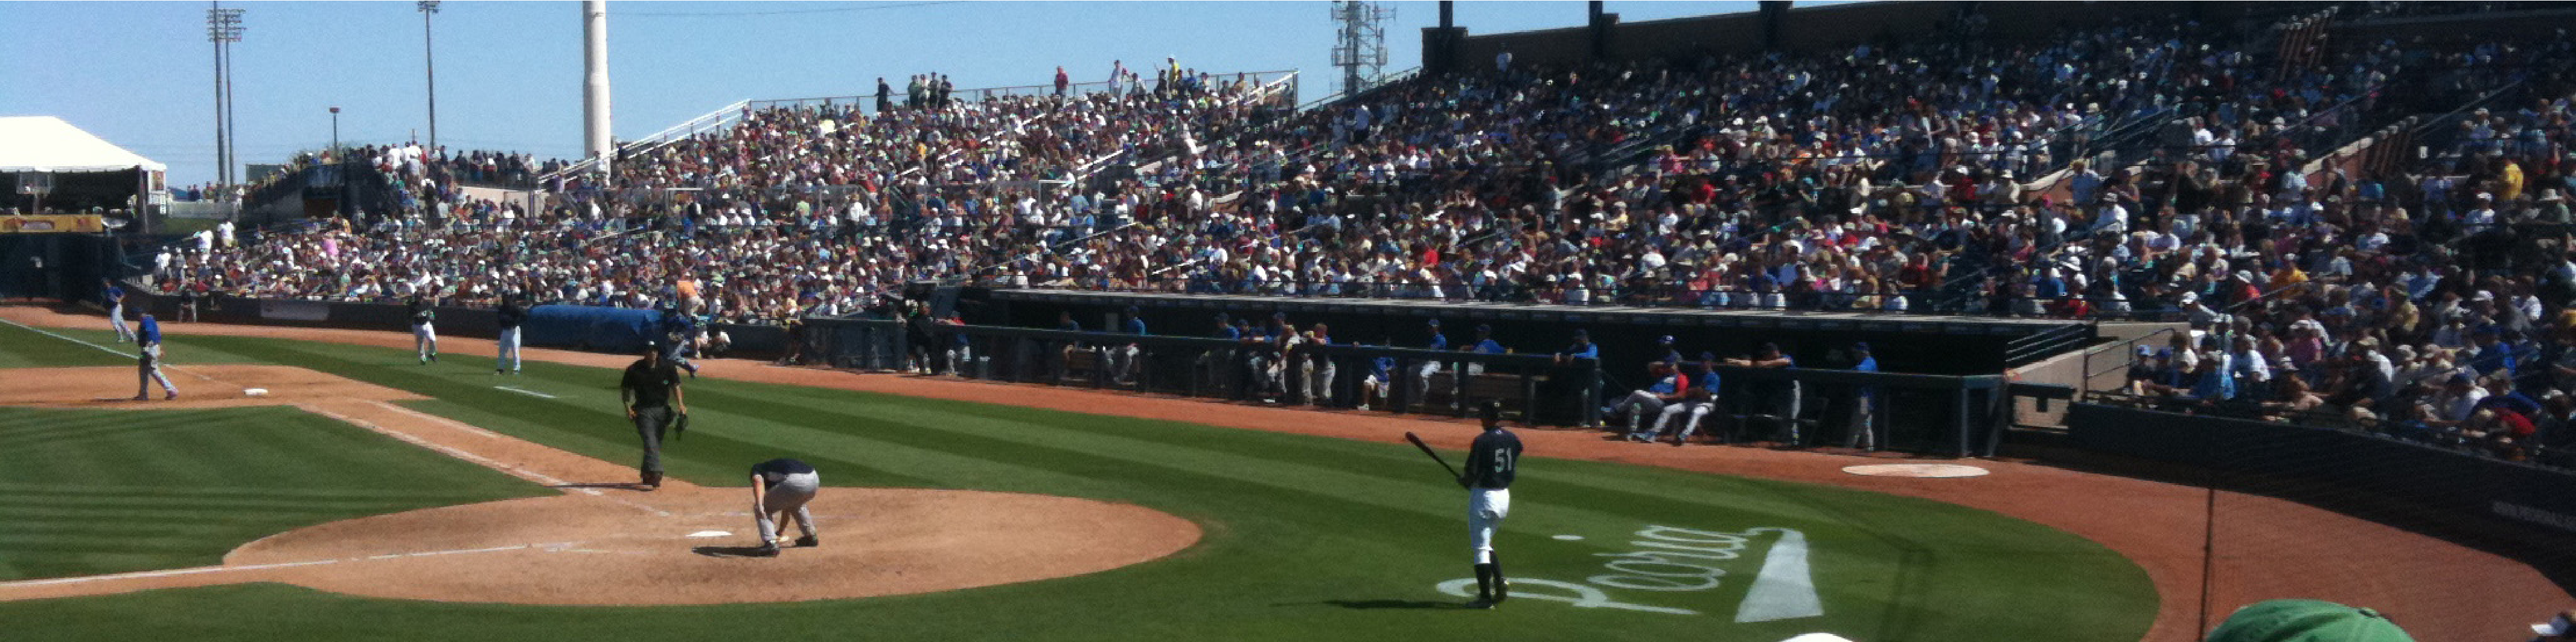
\includegraphics[width=\textwidth]{sampleteaser}
%   \caption{Seattle Mariners at Spring Training, 2010.}
%   \Description{Enjoying the baseball game from the third-base
%   seats. Ichiro Suzuki preparing to bat.}
%   \label{fig:teaser}
% \end{teaserfigure}

%%
%% This command processes the author and affiliation and title
%% information and builds the first part of the formatted document.
\maketitle

\section{Introduction}
\label{sec:introduction}
There are various types of helmets, such as industrial protective helmets, motorcycle and bicycle helmets, sports helmets (for American football, baseball, ice hockey, etc.), and military/police helmets. These are all worn to protect the head in the event of an accident \cite{helmet}. From a safety point of view, it is important that there is no gap between the head and the helmet.\par

Workers in factories and disaster sites must also often wear helmets. Wearing a helmet can allow individuals who do not know each other, such as classroom use is granted without fee provided that copies are not made or distributed short-term workers and vendors, to be identified by displaying their names and work division on their helmets. Helmets can also allow wearers to be identified from a distance or overhead even if their faces cannot be clearly seen. Identifying individuals also serves as a deterrent to trespassers. In addition, displaying qualifications, such as a hazardous materials engineer's license and a heavy machinery license, can help create a safe work environment. In many cases, this information is written directly on the helmet, or an identifiable sticker is attached to the helmet. However, such an analog system makes it possible for trespassers to easily disguise themselves by forging or stealing a sticker. In addition, a worker can put on another worker's helmet without being aware of it, and incorrect information will be displayed. If helmets are shared among workers, they are not marked with identifiable information.\par

In this paper, we propose a method that identifies users based on the shape of their heads by installing pressure sensors inside a helmet. We implemented a prototype helmet with 32 pressure sensors. Our method calculates the similarity between the wearer's data and registered users' data and outputs the user with the most similar data.\par

The prototype helmet has a display to indicate the user's name and credentials based on the identification results; therefore, incorrect information is not displayed on the helmet if a helmet belonging to someone else is used. One advantage of this system is that identification information is automatically displayed on a shared helmet, allowing workers to identify each other. Another advantage of user identification is data annotation. Data collected by sensors attached to the helmet or wearer's body, such as a camera, eye tracker, and accelerometer, can be automatically annotated with the wearer's ID. By attaching a Global Positioning System (GPS) module or antenna to localize the user \cite{disaster_en}, the name and location of a worker can be determined in real time, allowing the foreperson to have a better understanding of the overall situation in the field. Furthermore, from the pressure data between the helmet and the head, it is possible to verify whether the shape of the head matches the helmet, as a zero pressure value signifies that there is a gap between the helmet and head. Another potential use of the proposed helmet is to serve as a key to a room whose access is restricted based on one's position or qualifications.\par

%removed for 4p
%The proposed method has two functions: user identification and authentication. User identification is based on the assumption that a single helmet is shared by multiple individuals. The pressure sensor data of an individual who may wear a helmet are registered in advance, and an individual wearing a helmet is identified as one of the registered persons. Personal identification does not take into account that a non-registered individual may wear the helmet; if a non-registered individual wears the helmet, the identification result will be a registered user who has the most similar data to the wearer. User authentication determines whether the individual wearing the helmet is in fact the individual with the ID when the ID is provided to the system. We assume an environment in which all individuals have their own helmets (as in smartphone authentication). In addition, we assume an environment in which the user ID is entered when using a shared helmet (as in automated teller machine [ATM] authentication). Even if an intruder wears a helmet and enters a stolen ID, he or she can be identified as an intruder (authentication denied) because the head shape differs from that of the individual with the ID.\par

%The remainder of this paper is organized as follows. Section \ref{sec:related} introduces related work, Section \ref{sec:method} describes the proposed method, Section \ref{sec:evaluation} evaluates the proposed method, and Section \ref{sec:conclusion} concludes the paper.


\section{Related Work}
\label{sec:related}

\subsection{User Authentication Method}
There are several methods for identifying individuals: password, personal identification number (PIN), and stroke pattern; physical characteristics, such as face, fingerprint, voice print, and iris; and behavioral characteristics, such as handwriting and gait. However, passwords, PINs, and stroke patterns that can be freely set by individuals have a risk of spoofing by shoulder hacking, brute force attacks, and password duplication.\par

For physical characteristics, Chen et al. \cite{face_and_finger} proposed an authentication method using video images of the user's face and fingertips captured from the front and rear cameras of a mobile device. Siddharth et al. \cite{palm_print} proposed an authentication system based on the palm print and palm vein.
%The system uses visible and infrared light to acquire images of the palm print and palm vein, and authentication is performed by verifying the data against registration data in the database.
Sayo et al. \cite{lip_motion} proposed an authentication method based on a camera image that captures the shape of a user's lips (physical characteristic) and the movement of the lips during speech (behavioral characteristic). Another authentication method involving the mouth proposed Kim et al. \cite{teeth_and_voice} combines dental images and voice. Kouno et al. \cite{head_top_camera} proposed an image-based person identification system using depth images from an overhead camera. Bednarik et al. \cite{eye_movement} proposed an identification system that uses eye movements, such as pupil size and variation, gaze velocity, and the distance of the infrared reflection of the eye. Nogueira et al. \cite{finger_CNN} used convolutional neural networks for fingerprint authentication and achieved high classification accuracy.\par

With respect to behavioral characteristics, the authors proposed a method that authenticates smartphone users using acceleration sensor data from taking a smartphone out of their pockets \cite{murao_screen_unlock_blind}. Guerra-Casanova et al. \cite{accelerometer_authentification} proposed a method for authenticating users by the gestures of their hands using a mobile device with an embedded accelerometer. For motion-based authentication using accelerometers, it is possible to use the acceleration characteristics of motions before the helmet is put on for authentication by mounting an accelerometer on the helmet. However, there are various ways of putting on a helmet, such as putting it on in a hurry and taking care not to let the interior of the helmet become wet in the rain. Therefore, it is not practical to collect data from all individuals for various situations.\par

In this paper, we propose a method for identifying individuals by acquiring their head shape with pressure sensors while they wear a helmet. Our method does not require individuals to perform special behaviors or remain stationary for identification. With a wearable approach, our method can be used at any place and time. To breach the system, the exact three-dimensional shape of a person's head is required, which is difficult to replicate.


\subsection{Head State Recognition}
Toth et al. \cite{facial_expression_headset} focused on facial muscle signals, and six different facial expressions were classified using muscle signals and gyroscope values that were obtained from a low-cost off-the-shelf electroencephalogram (EEG) headset. EEG headsets are generally used to measure brain waves; however, muscle signals are detected locally because the measurement is performed by placing electrodes on the scalp.
%This method only uses existing EEG devices for the classification of facial expressions, and no additional electromyography sensors are used.
Kwon et al. \cite{facial_expression_glasses} designed a glasses-type wearable device to detect a user's emotions based on facial expressions and physiological reactions. The device can capture facial expressions with a built-in camera and detect physiological responses, such as photoplethysmogram signals and electrodermal activity. Fukumoto et al. \cite{fukumoto} designed a smile-based life-logging system that focuses on smile and laughter to index interesting or enjoyable events on recorded video. They used photointerrupters.\par
%, and smile/laughter was detected separately by threshold-based clustering. The evaluation results demonstrated a 73–94\% accuracy in detecting smile/laughter during actual use of the system.\par

These studies all use dynamic information, such as facial expressions and physical movements in the facial area. In contrast, our study uses static features of head shape.


\section{Proposed Method}
\label{sec:method}
In this section, we present the details of the proposed method.

\subsection{Overview}
The proposed method assumes that a user wears a helmet equipped with pressure sensors. It then acquires the shape of the wearer's head and determines whether the wearer is a registered user. The proposed method has two functions: user identification and authentication.
\begin{itemize}
    \item {\bf User identification} assumes that a single helmet is shared by multiple people and that no other information, such as the ID, is provided to the system; the user simply puts on the helmet. Users' pressure sensor data are registered in advance, and a user who puts on a helmet is identified as one of the registered users. User identification does not consider that a non-registered person may put on the helmet. If a non-registered person puts on the device, the identification result will be an individual with the closest data among the registered users.
    
    \item {\bf User authentication} determines whether the individual wearing the helmet is the correct individual when his/her ID or username is provided. We assume two cases in which authentication is used: (i) each individual has his/her own helmet and only the individual's pressure sensor data have been registered (single user; username is preset on device, as in smartphone authentication); and (ii) a helmet is shared among multiple users, and a username is entered when putting on the helmet (multiple users; usernames are input manually, as in ATM authentication). The pressure sensor data are registered in advance, and a user who puts on the helmet is accepted or rejected by calculating the similarity between the input data and the data corresponding to the ID. Even if the ID is leaked, an intruder can be rejected if his/her head shape differs from the data corresponding to the ID.
\end{itemize}

The flow of our system is illustrated in \figref{system}. A total of 32 pressure sensors are attached to the inner side of the helmet to acquire data, producing one-dimensional 32-channel pressure data. Pressure data of individuals who are expected to wear helmets are registered in the system in advance and are called training data in this paper. In user identification, the proposed system uses a support vector machine (SVM) to build a recognition model from the feature values extracted from the training data and outputs the identification results from the features of the input data of an unknown registrant. In user authentication, the system calculates the Mahalanobis distance between the training and input data of the user, including non-registrants, and authenticates the user if the distance is less than the threshold; otherwise, the user is rejected.

\begin{figure}[!t]
  \centering
    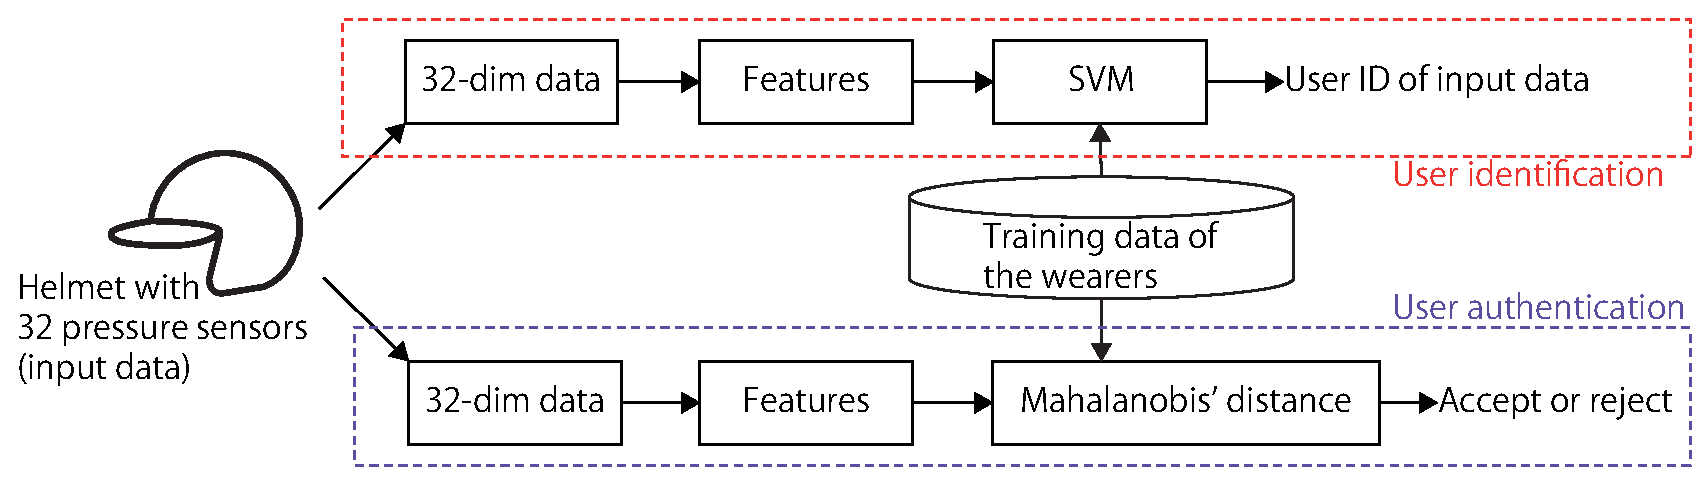
\includegraphics[width=1\linewidth]{figure/system.eps}
  \caption{Process of user identification and authentication.}
  \label{fig:system}
\end{figure}


\subsection{Hardware}
\label{sec:hardware}
We developed a helmet equipped with 32 pressure sensors as illustrated in \figref{hard}.
%\figref{device} presents the configuration of the device, and \figref{met_over} provides an image of the device. The head of the user must be in close contact with the sensors to obtain the correct pressure values; therefore,
We used a commercially available full-face helmet. The pressure sensors were FSR402 and FSR402 Short Tail manufactured by Interlink Electronics, Inc. The Arduino MEGA2560 R3 was used as a microcomputer. We installed a thick urethane sponge and inserted pressure sensors into the cut line of the sponge.\par
%Because the helmets was difficult to attach and remove the interior, we removed the interior of the top of the helmet and installed a thick urethane sponge, as illustrated in \figref{met_in}. The urethane sponge was cut and a pressure sensor was inserted into the cut line, as illustrated in \figref{sensor}.\par

Four pressure sensors were placed at the top of the head, 16 sensors were placed around the top of the head, six sensors were placed at the back of the head, and six sensors were placed at the cheek pads on both sides as displayed in \figref{position}.
%A total of 32 sensors were installed at the points, as displayed in \figref{position}.
The wiring for the pressure sensors passed through a hole drilled at the top of the helmet. The PCB and a display were bolted to both of the cheek area using a threaded hole drilled to secure the helmet shield, and was fixed and removable.
%and was then connected to a 5V power supply port, GND, and analog input port, which was on the Arduino MEGA2560 R3 via a printed circuit board (PCB) with a 10K$\Omega$ resistor that was mounted outside the helmet. \textcolor{blue}{The PCB and a display to show ID attached to the exterior of the helmet are illustrated in \figref{print} and \figref{lcd}. The PCB and a display were bolted to both of the cheek area using a threaded hole drilled to secure the helmet shield, and was fixed and removable.}

\begin{figure}[!t]
    \centering
    \includegraphics[width=1\linewidth]{figure/hardware.eps}
  \caption{Prototype helmet with 32 pressure sensors.}
  \label{fig:hard}
\end{figure}

\begin{figure}[!t]
  \begin{center}
    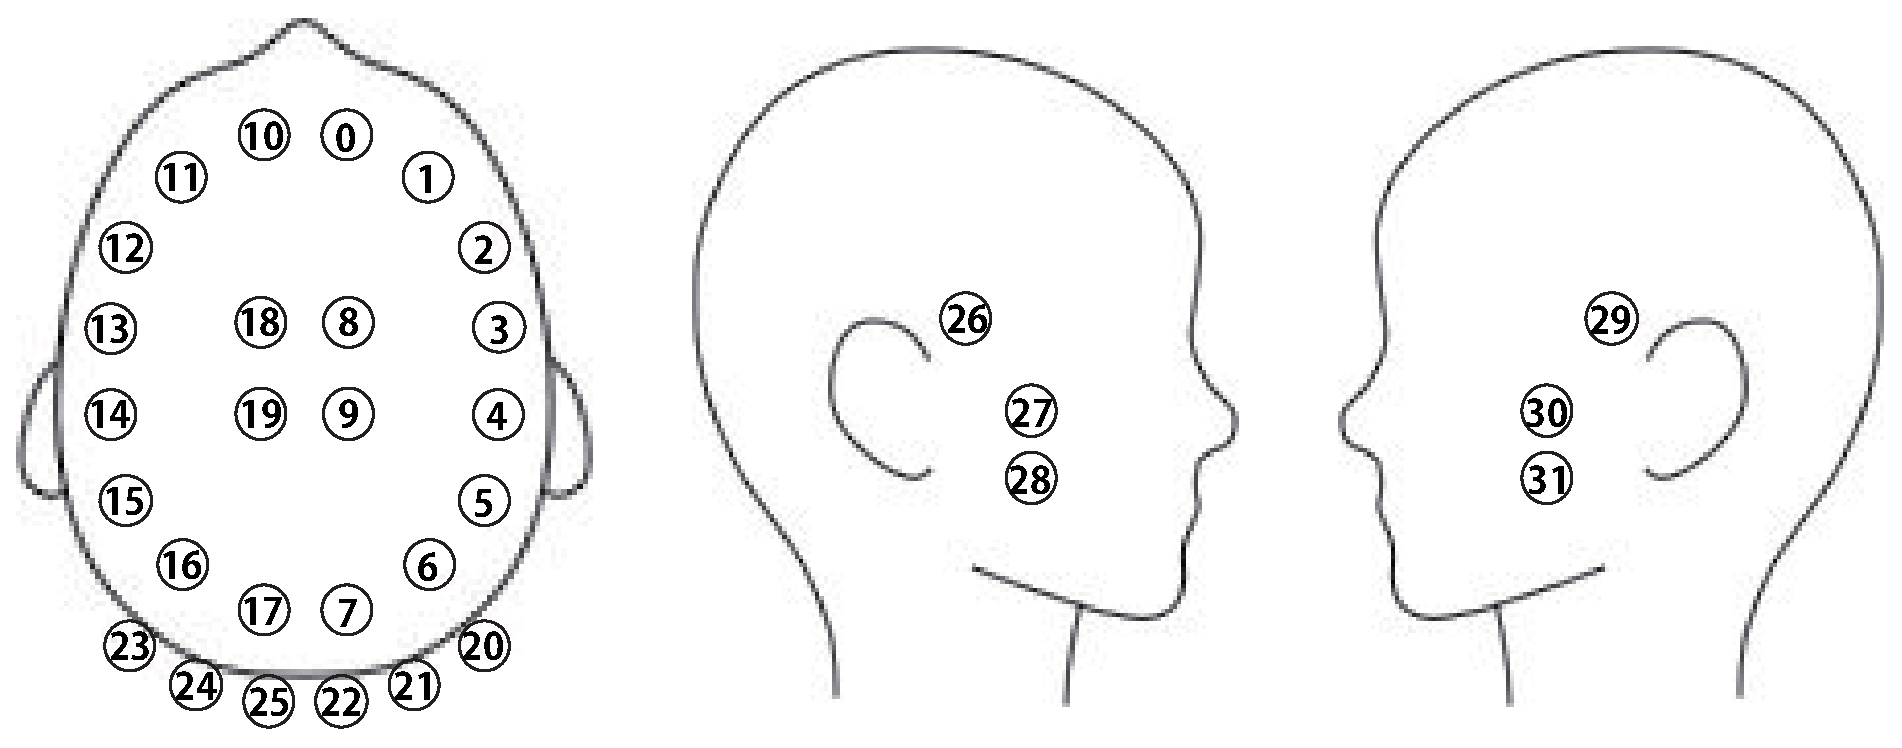
\includegraphics[width=1\linewidth]{figure/position.eps}
  \end{center}
  \caption{Position of pressure sensors.}
  \label{fig:position}
\end{figure}


\subsection{User Identification Method}

\subsubsection{Preprocessing.}
Data acquisition begins when a user puts on the helmet. Data from 32 pressure sensors $\bm{p}(t)=[p_1(t),\cdots,p_{32}(t)]$ are acquired at time $t$. The voltage values of all pressure sensors are almost 5V when the helmet is not worn, then sum of the data show $\sum_{i=1}^{32}p_i(t)\approx160[V]$. When the helmet is worn, $p_i(t)$ decreases, and the system segments the data over a 2-s window starting from $t=T_s$ after the values are stabilized. Time $t=T_s$ is the time at which the change of the sum of 32 dimensions per sample is less than 2V for 11 consecutive samples ($\approx$11/30 second as the sampling rate is approximately 30 Hz) after the sum of 32 dimensions is less than 155V, i.e. $\sum_{i=1}^{32}|p_i(t)-p_i(t-1)|<2[V]~(i=T_s,\cdots,T_s-10)$. The average value over the window $x_i(t)=\frac{1}{N}\sum_{t=T_S}^{T_S+N-1}p_i(t)$ for sensor channel $i$ ($i=1,\cdots,32)$ is calculated, where $N$ is the number of samples in the window. We then obtain a 32-dimensional vector $\bm{x}(t)=[x_{1}(t),\dots,p_{32}(t)]$ as a feature. Once the data is segmented, the preprocessing is suspended until $\sum_{i=1}^{32}p_i(t)>159$[V] is met.


\subsubsection{Identification.}
Given training data $[\bm{x}_m,y_m]$ $(m=1,\dots, M)$ from users who are expected to use the helmet by wearing the helmet a total of $M$ times in advance, the SVM is trained with the training data, where $y_m$ is the registrant label, such as the registrant's name and number. The input data $\bm{x}_{test}$ collected by the user to be identified are fed into the SVM and the classification result $\hat{y}_{test}$ is obtained.


\subsection{User Authentication Method}
\subsubsection{Preprocessing.}
In user authentication, data from 32 pressure sensor data $\bm{p}(t)=[p_1(t),\cdots,p_{32}(t)]$ and the average $\bm{x}(t)=[x_{1}(t),\dots,p_{32}(t)]$ are obtained as a feature in the same manner as for user identification.


\subsubsection{Similarity calculation.}
In user authentication, there are two cases for using training data: data of a single user are used and data of multiple users are used. For single-user data, data of only a single user (e.g., owner of the helmet) are registered or data of multiple users are registered; however, the data of only one of the users whose ID is provided are used. For multiple-user data, data of multiple users who are expected to use the helmet are used. With training data $[\bm{x}_m,y_m]$ $(m=1,\dots, M)$ obtained from user(s) wearing the helmet $M$ times in advance, the proposed method calculates the Mahalanobis distance, where $y_m$ is the registrant label, such as the registrant's name and number.\par

The Mahalanobis distance is a method for calculating the distance between multiple variables, and can be normalized considering the distribution of the data. The mean vector $\bm{\mu}$ and the variance-covariance matrix $\bm{\Sigma}$ of the training data are calculated by (\ref{eqn:mu}) and (\ref{eqn:sigma}).
\begin{eqnarray}
\label{eqn:mu}
  \bm{\mu} &=& \frac{1}{M}\sum_{m=1}^{M}\bm{x}_m \\
\label{eqn:sigma}
  \Sigma_{i,j} &=& \frac{1}{M}\sum_{m=1}^{M}(\bm{x}_i-\bm{\mu})(\bm{x}_j-\bm{\mu})^T
\end{eqnarray}
 
The Mahalanobis distance between the training data $\bm{x}_m$ $(m=1,\dots, M)$ and input data $\bm{x}_{test}$ can be calculated by (\ref{eqn:mahalanobis}).
\begin{eqnarray}
\label{eqn:mahalanobis}
  d(\bm{x},\bm{x}_m) = \sqrt{(\bm{x}-\bm{x}_m)^{T}\bm{\Sigma}^{-1}(\bm{x}-\bm{x}_m)}
\end{eqnarray}
If the input data are collected from a pre-registered user, the input data $\bm{x}_{input}$ follow the probability distribution of the variance-covariance matrix $\bm{\Sigma}$.


\subsubsection{Authentication decision.}
Letting $\theta$ be the threshold value, a user is authenticated if (\ref{eqn:authentication}) is satisfied and is rejected if (\ref{eqn:authentication}) is not satisfied.
\begin{equation}
\label{eqn:authentication}
  \theta \geq \min_m(d(\bm{x}_{input},\bm{x}_m))~(m=1,\cdots,M)
\end{equation}


\subsection{Software}
%The Arduino MEGA program was implemented by Arduino IDE, and a computer program that received data from Arduino MEGA and saved it in comma-separated values format was implemented in Python.
A computer program to analyze the data was implemented in Python.\par

In user identification, for the SVM, \texttt{sklearn.svm.SVC} of the scikit-learn \cite{scikit-learn} library, which is an implementation of the standard soft margin SVM, was used. We also used \texttt{sklearn.model\_selecti}\\\texttt{on.cross\_val\_score} for cross-validation and \texttt{sklearn.model\_se}\\\texttt{lection.GridSearchCV} for grid search and evaluation.\par

In user authentication, the system computed the variance-covariance matrix using \texttt{sklearn.covariance.MinCovDet}. For calculation of the Mahalanobis distance, \texttt{scipy.spatial.distance} was used. The minimum covariance determinant (MCD) is an algorithm that is robust to outlier values for estimating a variance-covariance matrix. \texttt{sklearn.covariance.MinCovDet} is a scikit-learn library that implement Fast-MCD \cite{fast_mcd}, a faster version of MCD. \texttt{scipy.spatial.}\\\texttt{distance} is a SciPy \cite{scipy} library that implements functions for calculating various distances.


\section{Evaluation}
\label{sec:evaluation}
This section describes the experiments conducted to evaluate the effectiveness of the proposed method.


\subsection{Data Collection}
We instructed nine subjects (A$\sim$I, all male, mean age 23 years) to wear the helmet implemented in Section \ref{sec:method} and collected sensor data. The sampling rate was approximately 30 Hz. The subjects put the helmet on for 2 s to collect data, then took it off and put it on again for 2 s to collect data, through which a set of two samples was obtained. By collecting data of 10 sets (20 samples) from each subject, a total of 180 samples (2 s $\times$ 20 samples $\times$ 9 subjects) were collected. Up to four sets of data were collected per person per day. To collect data for various positions of the sensors and head, a rest period of at least 30 minutes was provided between sets.


\subsection{User Identification Method}
\subsubsection{Evaluation environment.}
We evaluated the proposed method using 5-fold cross-validation in which 80\% of the data (16 samples) collected from each subject were trained and 20\% (four samples) were tested. To investigate the effect of the number of sensors used, the identification accuracy for all combinations of sensors from 1–32 sensors was measured.\par

To simulate a half helmet, which is commonly used at construction sites, the identification accuracy for all combinations of sensors from 1 to 20 sensors limited in the top half out of 32 sensors were measured. These 20 sensors are sensors \#0--\#19 in \figref{position}. In this evaluation, two types of sensor configurations were tested: a full-face helmet with 32 sensors and a half helmet with 20 sensors.


\begin{table*}[!t]
\tabcolsep=1.5mm
\centering
  \begin{tabular}{cccc}

  \begin{minipage}[c]{.20\linewidth}
  \centering
  \caption{Identification accuracy with a full-face helmet, where the number of sensors was reduced from 32 to 1.}
  \begin{tabular}{l|c} \hline\hline
    Sensors used & Accuracy \\ \hline
    32 sensors & 1.000 \\
    31 sensors & 1.000 \\
    \vdots & \vdots \\
    5 sensors & 1.000 \\
    $\#$0, $\#$3, $\#$5, $\#$16 & 0.994 \\
    $\#$3, $\#$11, $\#$24       & 0.972 \\
    $\#$3, $\#$25               & 0.922 \\
    $\#$10                      & 0.617 \\ \hline
  \end{tabular}
  \label{tab:full_num}
  \end{minipage}&
  \begin{minipage}[c]{.20\linewidth}
  \centering
  \caption{Identification accuracy with a half helmet, where the number of sensors was reduced from 20 to 1.}
  \begin{tabular}{l|c} \hline\hline
    Sensors used & Accuracy \\ \hline
    20 sensors & 1.000 \\
    19 sensors & 1.000 \\
    \vdots & \vdots \\
    5 sensors & 1.000 \\
    $\#$0, $\#$3, $\#$5, $\#$16 & 0.994 \\
    $\#$0, $\#$3, $\#$13        & 0.983 \\
    $\#$3, $\#$16               & 0.928 \\
    $\#$10                      & 0.617 \\ \hline
  \end{tabular}
  \label{tab:half_num}
  \end{minipage}&
  \begin{minipage}[c]{0.20\linewidth}
  \centering
  \caption{Equal error rate (EER) for subjects in user authentication.}
  \begin{tabular}{c|c} \hline\hline
    Subject & EER \\ \hline
    A & 0.002 \\
    B & 0.095 \\
    C & 0.050 \\
    D & 0.055 \\
    E & 0.006 \\
    F & 0.094 \\
    G & 0.012 \\
    H & 0.050 \\
    I & 0.000 \\ \hline
    Average & 0.076 \\ \hline
  \end{tabular}
  \label{tab:EER_num}
\end{minipage}&
\begin{minipage}[c]{0.34\linewidth}
\centering
  \centering
    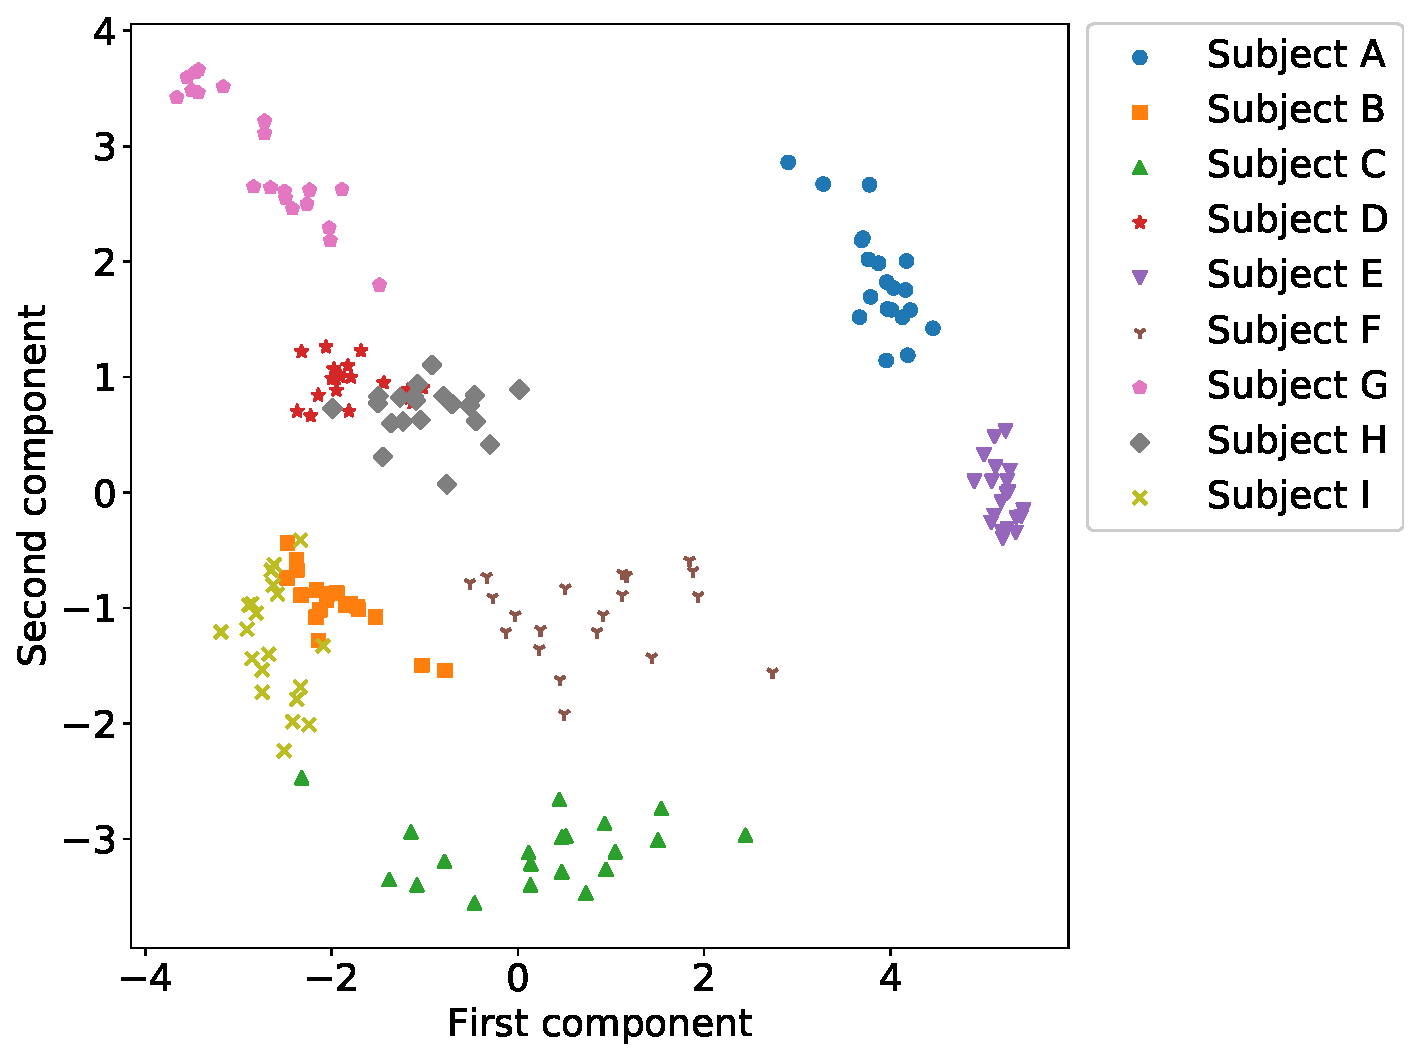
\includegraphics[width=1\linewidth]{figure/PCA.eps}
  \caption{Principal component distribution of 32-dimensional features compressed into two dimensions by principal component analysis.}
  \label{fig:PCA}
\end{minipage}
  
  \end{tabular}
\end{table*}


\subsubsection{Results and discussion.}
The accuracy of user identification with a full-face helmet and half helmet is presented in \tabref{full_num} and \tabref{half_num}. The numbers listed in the ``Sensors used'' column are the number of sensors in \figref{position}. For a full-face helmet, when the number of sensors was 32, the number of sensor combinations was 1 ($_{32}C_{32}=1$), and when the number of sensors was 31, the highest accuracy of $_{32}C_{31}=32$ combinations is presented in the table. For a half helmet, when the number of sensors was 20, the number of sensor combinations was 1, and when the number of sensor was 19, the highest accuracy of 20 combination is presented in the table. For one to four sensors, the regularization parameter of the SVM was set to $C=1.0$, and the sensor combination with the highest accuracy was recorded. Then, the best C was determined by grid search for the sensor combination, and the highest accuracy is presented in the tables.\par

We determined that the accuracy was 1.000 when 32 and 31 sensors were used for the full-face helmet and 20 and 19 sensors were used for the half helmet. Therefore, we measured the accuracy from one sensor until the accuracy reached 1.000 and skipped the measurement of the accuracy for additional sensors.\par

For the full-face helmet, nine subjects were identified with 100\% accuracy when five sensors were used. The accuracy was 99.4\% using four sensors, 97.2\% using three sensors, and 92.2\% using two sensors. However, the accuracy significantly decreased to 61.7\% using one sensor.\par

For the half helmet, nine subjects were identified with 100\% accuracy when five sensors were used. The accuracy was 99.4\% using four sensors, 98.3\% using three sensors, and 92.8\% using two sensors. However, the accuracy decreased significantly to 61.7\% when only one sensor was used.\par

Both the full-face helmet and half helmet achieved 100\% accuracy with at least five sensors for the dataset used in this experiment. However, the number of sensors required to achieve high accuracy may increase as the number of registrants increases. For the sensors used for the full-face helmet, most were numbered under \#20, signifying that sensors in the top half were significant.


\subsection{User Authentication Method}
\subsubsection{Evaluation environment.}
One subject was considered the individual to be authenticated (i.e., owner) while the remaining eight subjects were considered strangers. The authentication accuracy of the owner was measured using 5-fold cross-validation, where 80\% of the owner's data (16 samples) were registered as training data and the remaining 20\% of the data (four samples) were used as test data. In addition, the authentication accuracy for strangers was measured using data from all eight strangers (160 samples). All 160 samples were tested in each fold of the cross-validation, and all nine subjects were evaluated on a rotation basis.\par

In user authentication, the false rejection rate (FRR), false acceptance rate (FAR), and equal error rate (EER) were used as indicators of authentication accuracy.
%The FRR is the rate at which a registered user is mistakenly considered a stranger and rejected, whereas the FAR is the rate at which a stranger is mistakenly considered a registered user and authenticated.
The smaller the threshold value $\theta$ in \ref{eqn:authentication} is set, the stricter the authentication decision becomes, resulting in an increased FRR.
%In contrast, the larger the threshold value $\theta$ is set, the looser the authentication decision becomes, resulting in an increased FAR.
There is a trade-off between the FRR and FAR, and the value at which the FRR and FAR are equal is called the EER. The EER value is commonly used as an indicator to evaluate the performance of authentication methods, and a small EER indicates better performance.


\subsubsection{Results and discussion.}
The EER of each subject and the average is presented in \tabref{EER_num}.
%In this table, ``Average'' represents the average EER of all subjects. The FRR and FAR values for each subject by varying the thresholds from 0 to 60 by 1 are presented in \figref{EER}. In this figure, ``Average'' represents the average FRR and FAR of all subjects.
The EER of subjects A, E, G, and I was approximately 0.01 or lower, which signifies that the owner failed authentication less than once in 100 times and that strangers broke the authentication less than once in 100 times. An EER of 0.0097 for user authentication using ear acoustics was reported in Ref. \cite{ear_auth}; therefore, our method achieved comparable performance for four of nine subjects.\par

The next most accurate subjects were C, D, and H, with an EER of approximately 0.05. To determine the cause of the decline in accuracy compared with subjects A, E, G, I, all collected data were compressed to the first principal component and second principal component by principal component analysis (PCA). The results of the data plotted on a two-dimensional plane are presented in \figref{PCA}. The plots for subject C indicate that one sample of the data of subject C was close to the data of subject I and the variance in the first principal component was large, which would reduce the accuracy. Furthermore, the data for subjects D and H significantly overlapped with each other, which affected the accuracy of both subjects.\par

The least accurate subjects were B and F, with an EER of approximately 0.095. Data for subject B was some overlap with the data of subject I. However, the EER of subject I was 0, which indicates perfect authentication. Therefore, the overlap of these data groups was likely due to the loss of data when they were compressed into two dimensions by PCA. On the other hand, subject F's data did not exhibit any overlap with other subjects' data; however, there was a large variance in both directions for the first and second principal components. Considering the effect of data compression by PCA, duplication with other subjects' data groups can be inferred in the 32-dimensional data. The accuracy for subjects B and C, who had data groups located close to subject F's data groups, may have been affected by the scattered data of subject F. In particular, the accuracy of subject B was likely to be lower than that of subject C because the two samples of subject B were located in close proximity to subject F's data group.

%The data of subject E were located at the rightmost points. In addition, the variance was small, and the data were thus considered distinct. For subject E in \figref{EER}, the FRR and FAR crossed at a threshold of approximately 60, which was greater than for the other subjects. This is because the data were quite different from the others, and the FAR did not increase by increasing the threshold.\par

%In summary, the mean EER of all subjects in user authentication was approximately 0.076. It is necessary to validate with data from a larger number of subjects, as there was a difference in the EER between subjects. In addition, it is necessary to investigate a method for authentication using time series pressure data from the start of wearing the helmet to the complete of wearing.


\section{Conclusion}
\label{sec:conclusion}
In this study, we proposed a method to identify individuals based on differences in head shape, which was measured by wearing a helmet with pressure sensors. We implemented the prototype device and evaluated our proposed method with nine subjects.
%The prototype device was a commercially available full-face helmet, and we attached 32 pressure sensors inside the helmet. In the evaluation, we obtained sensor values for 2 s 20 times from nine subjects as head shape data. Using the acquired data, we evaluated the user identification accuracy to determine which user was wearing the helmet among the registrants. In addition, we evaluated the user authentication accuracy to determine whether the helmet wearer was the registrant.\par
As the accuracy was 100\% with 32 sensors in user identification, we tested how the accuracy changed by decreasing the number of sensors. The results indicated that the smallest number of sensors producing 100\% accuracy was five. The EER of four out of nine subjects was less than 0.012, and the average EER in authentication was 0.076.
%These results suggest that our method is effective as a user identification method. In the future, we will collect additional data and evaluate the proposed method in a real environment.




%%
%% The next two lines define the bibliography style to be used, and
%% the bibliography file.
\bibliographystyle{ACM-Reference-Format}
\bibliography{references}

% %%
% %% If your work has an appendix, this is the place to put it.
% \appendix

% \section{Research Methods}

% \subsection{Part One}

% Lorem ipsum dolor sit amet, consectetur adipiscing elit. Morbi
% malesuada, quam in pulvinar varius, metus nunc fermentum urna, id
% sollicitudin purus odio sit amet enim. Aliquam ullamcorper eu ipsum
% vel mollis. Curabitur quis dictum nisl. Phasellus vel semper risus, et
% lacinia dolor. Integer ultricies commodo sem nec semper.

% \subsection{Part Two}

% Etiam commodo feugiat nisl pulvinar pellentesque. Etiam auctor sodales
% ligula, non varius nibh pulvinar semper. Suspendisse nec lectus non
% ipsum convallis congue hendrerit vitae sapien. Donec at laoreet
% eros. Vivamus non purus placerat, scelerisque diam eu, cursus
% ante. Etiam aliquam tortor auctor efficitur mattis.

% \section{Online Resources}

% Nam id fermentum dui. Suspendisse sagittis tortor a nulla mollis, in
% pulvinar ex pretium. Sed interdum orci quis metus euismod, et sagittis
% enim maximus. Vestibulum gravida massa ut felis suscipit
% congue. Quisque mattis elit a risus ultrices commodo venenatis eget
% dui. Etiam sagittis eleifend elementum.

% Nam interdum magna at lectus dignissim, ac dignissim lorem
% rhoncus. Maecenas eu arcu ac neque placerat aliquam. Nunc pulvinar
% massa et mattis lacinia.

\end{document}
\endinput
%%
%% End of file `sample-authordraft.tex'.
